\section{Application to path tracing}
\label{sec::appli_pathtrace}

In this section, we explain how the curvilinear skeleton of the voids of the scene can enhance the path tracing algorithm. We start with some basic elements related to path tracing and then present our modified path tracing algorithm.

%\subsection{Basic definitions of radiometry}
%
%Let $S$ be a set of surfaces of $\Rset^3$ that don't overlap and $S_L \subset S$ a set of surface lights. $S$ is called the scene.
%
%The basic radiometric quantity is the \myem{radiance} $L(x \rightarrow \Theta)$ that expresses the quantity of light energy produced by the surface point $x \in \Rset^3$ toward direction $\Theta \in \Omega_x$ per unit of time per unit area per unit solid angle (expressed in $W.m^{-2}.sr^{-1}$).
%This is the quantity that the eye actually "sees" and that must be computed for each pixel of the final image.
%
%% image radiance
%
%We can define another quantity related to radiance called \myem{incoming radiance} $L(x \leftarrow \Phi)$ that represents the radiance that reach $x$ from direction $\Phi$.
%
%In the void, incoming radiance can be written in terms of radiance as follow:
%
%\begin{equation*}
%L(x \leftarrow \Phi) = L(r(x, \Phi) \rightarrow -\Phi)
%\end{equation*}
%
%$r(x, \Phi)$ is the surface point seen by $x$ in the direction $\Phi$. It can be defined formally by:
%
%\begin{align*}
%r(x, \Phi) &= x + t_{min}\Phi \\
%t_{min} &= min \lbrace t \in (0, +\infty]~ |~ x + t\Phi \in S \rbrace
%\end{align*}
%
%If $t_{min} = \infty$ then $r(x, \Phi)$ is undefined and $L(x \leftarrow \Phi) = 0$. We call $r$ the \myem{raytrace} function. In practice it is implemented by throwing a ray in the scene and looking for the first intersection.
%
%A third quantity related to radiance is \myem{emitted radiance} $L_e(x \rightarrow \Theta)$. It is not null if $x$ is a point of a light source ($x \in S_L$). In practice the emitted radiance is given with the set $S_L$ as an input of the algorithm.
%
%The radiance is the solution of an equation called the Rendering Equation:
%
%\begin{align*}
%L(x \rightarrow \Theta) &= L_e(x \rightarrow \Theta) + \int_{\Phi \in \Omega_x} f_r(x, \Theta \leftrightarrow \Phi) L(x \leftarrow \Phi) cos(N_x, \Phi) d\omega_\Phi \\
%&= L_e(x \rightarrow \Theta) + L_r(x \rightarrow \Theta)
%\end{align*}
%
%This equation expresses an intuitive idea: the radiance produced by the point $x$ in the direction $\Theta$ is the sum of the emitted radiance and the reflected radiance.  The reflected radiance is computed by integrating the incoming radiance scaled by a factor $f_r(x, \Theta \leftrightarrow \Phi) cos(N_x, \Phi)$ over all the possible directions of the hemisphere around $x$. $N_x$ is the surface normal at point $x$.
%
%The $f_r$ function is called the \myem{bidirectional reflectance function} (BRDF) and express the exchange of radiance between the incoming direction $\Phi$ and the output direction $\Theta$. Intuitively it represents the material properties of the surface at point $x$. A mirror doesn't reflect light the same manners a wall do, the BRDF encodes that.
%
%It's actually the rendering equation that a path tracer try to resolve. Let $O$ be the origin of the camera and $I$ the image we want to compute (a rectangle embedded in $\Rset^3$). Then the path tracing algorithm compute an approximation of the radiances $L(O \leftarrow \vec{OP})$, $\forall P \in I$.

\subsection{The path tracing}

Let $O$ be the origin of the camera in the scene. For each pixel $P$ of the final image, let $x$ be the nearest intersection point of the ray $(O, \overrightarrow{OP} = -\Theta)$ with an element of the scene. To obtain the luminosity, we must solve the rendering equation \cite{Ka86} which is a recursive integral equation, the integrand containing the radiance function that we must compute:
\begin{center}
$L(x \rightarrow \Theta) = L_e(x \rightarrow \Theta) + \int_{\Phi \in \Omega_x} f_s(x, \Theta \leftrightarrow \Phi) L(r(x, \Phi) \rightarrow -\Phi) d\omega_\Phi$
\end{center}
where $L$ is the radiance (a radiometric quantity that represents luminosity) from point $x$ toward direction $\Theta$ and $L_e$ is the emitted radiance (non null only on light sources). The point $r(x, \Phi)$ is the nearest visible point from $x$ in the direction $\Phi$ of the hemisphere $\Omega_x$. The $f_s$ function expresses how much luminosity is exchanged, on point $x$, between an incoming ray $\Phi$ and the outgoing ray $\Theta$.

The previous equation expresses an intuitive idea: the reflected radiance from $x$ towards the camera is the result of computing all incoming luminosity on $x$ scaled by a factor which depends on the material on $x$ and the angle of the ray going from the camera to $x$. The most common method used to estimate the integral, denoted by $L_r(x \rightarrow \Theta)$, is the Monte-Carlo integration which provides the following:

\begin{equation*}
\langle L_r(x \rightarrow \Theta) \rangle = \frac{f_s(x, \Theta \leftrightarrow \Phi) L(r(x, \Phi) \rightarrow -\Phi)}{p(\Phi)}
\end{equation*}

The function $p$ is a probability density function (pdf) that is used to sample $\Phi$. This estimator is unbiased, meaning that the expected value $E[\langle L_r(x \rightarrow \Theta) \rangle]$ is equal to $L_r(x \rightarrow \Theta)$. The variance of the estimator expresses its quality and depends on the chosen pdf $p$. The best choice is a pdf that matches the shape of the function to integrate (ie. gives high density to samples that have high values for the function and low density to samples that have low values).
The strategy of choosing an adapted pdf is called \myem{importance sampling}~\cite{Ka86} and is used in global illumination to improve the convergence speed of the algorithms.

The algorithm computes $L$ as follow: it chooses one random direction $\Phi$ based on the pdf $p$ and applies the estimator by calling $L$ recursively to compute $L_r$ (shoots a new ray in the direction $\Phi$, computes the new hit point with the scene, and compute the new radiance at this point). Finally, it returns the sum of the emitted radiance $L_e$ and the result for $L_r$. The recursion stops when either a maximal number of bounces or a directly illuminated area have been reached.

This computation is done multiple times for each pixel. We average the results and get an estimation of the mean radiance passing through the pixel and heading towards the camera.
A bad pdf would lead in picking directions that do not reach the light before the end of the recursion, and produce results with a lot of noise in the final image. In the next part, we explain how to produce a pdf based on the curvilinear skeleton.


\subsection{Skeleton based importance sampling}

As stated in the introduction, a curvilinear skeleton of the void (with some preprocessing performed on it) gives us information on which directions the light comes from. Given these directions, we can build a efficient pdf $p_{skel}$ and guide our rays by sampling the hemispheres with $p_{skel}$. The integrand of $L_r$ is:

\begin{equation*}
f_s(x, \Theta \leftrightarrow \Phi) L(r(x, \Phi) \rightarrow -\Phi).
\end{equation*}

The most common strategy used to sample $\Omega_x$ is to use the function $f_s$ because it is an input of the algorithm.
The term $L$, representing the distribution of light in the scene, is unknown. Our method gives a way to sample $L$.


\subsubsection{Construction of the importance points}

The skeleton of the voids of the scene is computed using Alg.~\ref{algo::3d_curvskel} (as shown on Fig.~\ref{fig::example_imp} on the right) and is converted to a graph (the nodes are the 0-faces and the edges are the 1-faces). We then compute a set of \myem{importance points}, which will be used to sample $\Omega_x$ in the path tracing algorithm. To each node $n$ of the skeleton, one importance point $imp_n$ is computed. Intuitively, the importance point associated to $n$ is the direction to follow in order to find a light source.

%La, pas clair !!!
Let $L$ be the light source of the scene and $n_L$ the nearest node of the skeleton that is visible by $L$. For each node, we compute the shortest path to $n_L$ along the skeleton. To do so, we use the Dijkstra algorithm and weight the edges of the skeleton depending on a visibility criteria: the weight of an edge $e$ is $1$ if $e$ is visible from $n_L$ and $10$ else. It results that illuminated paths will be shorter than paths located in dark areas.

Let $n$ be a node of the skeleton and $V_n$ the set of visible nodes from $n$ along the shortest path toward $n_L$. The importance point $imp_n$ associated to $n$ is the barycenter of $V_n$. An example is shown on Fig.~\ref{fig::example_imp} on the left.
The algorithm can be extended to multiple light sources by taking into account, when computing the importance point of a skeleton node, only the closest light source.




\subsubsection{Sampling according to $L$}

Given a point $x$ on the scene and a direction $\Theta$, we want to compute $L(x \rightarrow \Theta)$ and then sample the hemisphere $\Omega_x$. We search for the nearest skeleton node $n$ to $x$ and its importance point $imp_n$. We sample the hemisphere with a power-cosine pdf centered on $\overrightarrow{x\,imp_n}$:
\begin{center}
$p_{skel}(\Phi) = \frac{s + 1}{2\pi}  * cos^s \alpha$
\end{center}
with $\alpha$ the angle between $\overrightarrow{x\,imp_n}$ and $\Phi$, $s$ being a parameter called skeleton strength. The higher $s$ is, the closer to $\overrightarrow{x\,imp_n}$ we sample.


\subsection{Results and discussion}
Some results are presented on Fig.~\ref{fig:results} and Fig.~\ref{fig::intro_image} where we can see that our method produces less noisy images compared to the regular path tracing. We present, in Fig~\ref{tab:timing}, the time taken by each method to produce an image of same quality (the quality is measured by the mean square error (MSE) with a reference image) in different scenes: our method is the fastest.



\section{Conclusion}
We presented in this article a new skeletonization algorithm that both preserves geometrical features of objects and produces a pure curvilinear skeleton. These two properties allow us to improve the path tracing algorithm in guiding the rays towards the main illuminated area of the scene. Our algorithm is faster and produce less noise than the classical path tracing method.


\begin{figure}[t]
\begin{center}
\begin{tabular}{l|r}
	\myincludegraphics{0.3\textwidth}{graph_heuristic.pdf} ~~~~~~&
	~~~~~~ \myincludegraphics{0.6\textwidth}{skel.jpg} \\
\end{tabular}
\caption[Example of importance point construction]{\label{fig::example_imp} \textbf{On the left}, we illustrate the importance point $imp_n$ associated to a node $n$. The dotted black line shows the closest node to $n$ not included in $V_n$. \textbf{On the right}, an example of the curvilinear skeleton (in red) obtained in the Sponza scene.}
\end{center}
\end{figure}


\begin{figure}[t]
\begin{center}
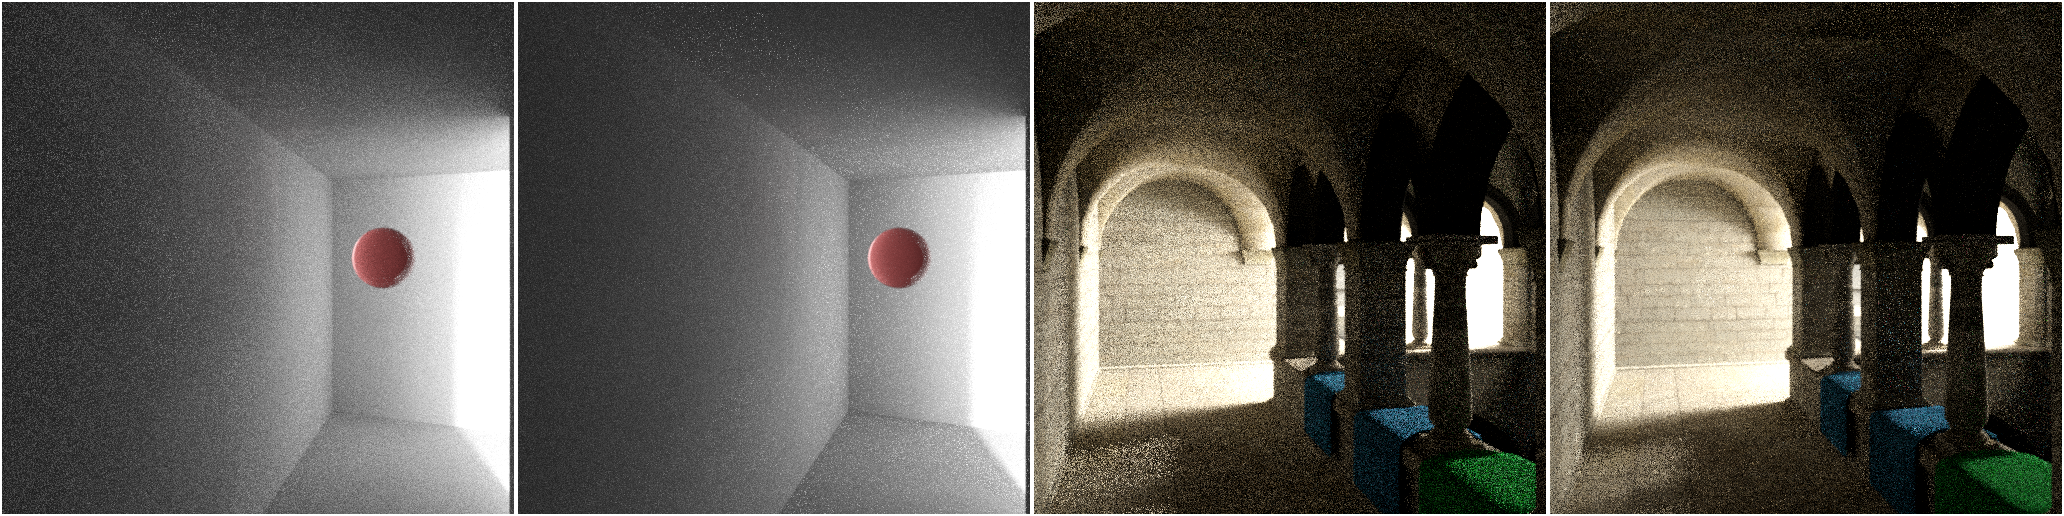
\includegraphics[scale=0.17]{images/four_scenes_for_dgci.png}
\caption{\label{fig:results}Same scene rendered using the classical path tracing (image $a$) or our method (image $b$). Images $c$ and $d$ are both details of respectively images $a$ and $b$ }
\end{center}
\end{figure}

\begin{figure}[tb]
\centering
\begin{tabular}{|c|c|c|c|}
\hline
Scene & Corridor & Sponza 1 & Sponza 2 (Fig. \ref{fig:results}) \\
\hline
MSE 100& 145 / 57 & 301 / 156 & 881 / 826 \\
\hline
MSE 40& 434 / 260 & 924 / 628 & 2678 / 2570 \\
\hline
\end{tabular}
\caption{Time (s) to reach an MSE of 100 and 40 against reference images. In each cell, the left number is for the standard path tracing, the right is for our method}
\label{tab:timing}
\end{figure}